% Options for packages loaded elsewhere
\PassOptionsToPackage{unicode}{hyperref}
\PassOptionsToPackage{hyphens}{url}
%
\documentclass[
]{book}
\usepackage{amsmath,amssymb}
\usepackage{iftex}
\ifPDFTeX
  \usepackage[T1]{fontenc}
  \usepackage[utf8]{inputenc}
  \usepackage{textcomp} % provide euro and other symbols
\else % if luatex or xetex
  \usepackage{unicode-math} % this also loads fontspec
  \defaultfontfeatures{Scale=MatchLowercase}
  \defaultfontfeatures[\rmfamily]{Ligatures=TeX,Scale=1}
\fi
\usepackage{lmodern}
\ifPDFTeX\else
  % xetex/luatex font selection
\fi
% Use upquote if available, for straight quotes in verbatim environments
\IfFileExists{upquote.sty}{\usepackage{upquote}}{}
\IfFileExists{microtype.sty}{% use microtype if available
  \usepackage[]{microtype}
  \UseMicrotypeSet[protrusion]{basicmath} % disable protrusion for tt fonts
}{}
\makeatletter
\@ifundefined{KOMAClassName}{% if non-KOMA class
  \IfFileExists{parskip.sty}{%
    \usepackage{parskip}
  }{% else
    \setlength{\parindent}{0pt}
    \setlength{\parskip}{6pt plus 2pt minus 1pt}}
}{% if KOMA class
  \KOMAoptions{parskip=half}}
\makeatother
\usepackage{xcolor}
\usepackage{longtable,booktabs,array}
\usepackage{calc} % for calculating minipage widths
% Correct order of tables after \paragraph or \subparagraph
\usepackage{etoolbox}
\makeatletter
\patchcmd\longtable{\par}{\if@noskipsec\mbox{}\fi\par}{}{}
\makeatother
% Allow footnotes in longtable head/foot
\IfFileExists{footnotehyper.sty}{\usepackage{footnotehyper}}{\usepackage{footnote}}
\makesavenoteenv{longtable}
\usepackage{graphicx}
\makeatletter
\def\maxwidth{\ifdim\Gin@nat@width>\linewidth\linewidth\else\Gin@nat@width\fi}
\def\maxheight{\ifdim\Gin@nat@height>\textheight\textheight\else\Gin@nat@height\fi}
\makeatother
% Scale images if necessary, so that they will not overflow the page
% margins by default, and it is still possible to overwrite the defaults
% using explicit options in \includegraphics[width, height, ...]{}
\setkeys{Gin}{width=\maxwidth,height=\maxheight,keepaspectratio}
% Set default figure placement to htbp
\makeatletter
\def\fps@figure{htbp}
\makeatother
\setlength{\emergencystretch}{3em} % prevent overfull lines
\providecommand{\tightlist}{%
  \setlength{\itemsep}{0pt}\setlength{\parskip}{0pt}}
\setcounter{secnumdepth}{5}
\usepackage{booktabs}
\ifLuaTeX
  \usepackage{selnolig}  % disable illegal ligatures
\fi
\IfFileExists{bookmark.sty}{\usepackage{bookmark}}{\usepackage{hyperref}}
\IfFileExists{xurl.sty}{\usepackage{xurl}}{} % add URL line breaks if available
\urlstyle{same}
\hypersetup{
  pdftitle={Fishnet2 Data Migration},
  pdfauthor={Jeremy Holden},
  hidelinks,
  pdfcreator={LaTeX via pandoc}}

\title{Fishnet2 Data Migration}
\author{Jeremy Holden}
\date{2023-07-06}

\begin{document}
\maketitle

{
\setcounter{tocdepth}{1}
\tableofcontents
}
\hypertarget{about}{%
\chapter{About}\label{about}}

The goal of this project is to document the workflow of migrating FN2 projects from the existing \emph{DATA.ZIP} archive to a modern data product. The manual will outline tools for importing, cleaning and outputting a project or series of projects.

\hypertarget{usage}{%
\section{Usage}\label{usage}}

This manual will focus on the code and associated R packages used to migrate data.

\hypertarget{introduction}{%
\chapter{Introduction}\label{introduction}}

Fishnet2 (FN2) is custom database software used as a Ontario provincial standard for over two decades. The system applied a common database structure to accommodate a variety of fishery surveys (i.e.~gill net, trawl, creel).

\hypertarget{overview}{%
\section{Overview}\label{overview}}

The goal of this manual is to document the process used to develop an R-based reproducible workflow for importing, cleaning and migrating archived FishNet2 project data.

\hypertarget{basic-workflow}{%
\section{Basic workflow}\label{basic-workflow}}

\begin{enumerate}
\def\labelenumi{\arabic{enumi}.}
\tightlist
\item
  The R package development structure is used as a framework for organizing the files and workflow.
\item
  FN2 archive files store relational data tables in a DBF format in a compressed format (\emph{DATA.ZIP}). These files are unzipped to memory then read in to an R environment.\\
\item
  Data types are imported as \emph{strings} and are converted to usable data types (i.e.~\emph{integers}, \emph{dates}, \emph{double}).\\
\item
  Error checking and data correction is conducted using a series of predefined and project specific queries.\\
\item
  Data variables names are standardized across projects.\\
\item
  At this point the data can be used or distributed as an R data package.
\item
  Data can also be exported from the package to other database formats as needed.
\end{enumerate}

\hypertarget{why-use-r}{%
\section{Why use R?}\label{why-use-r}}

Generally, a code-based approach (R or other programming languages like Python) are advantageous over other graphic user interface (GUI) approaches that rely on point-and-click actions that are often not documented and are certainly not reproducible. The primary advantage of using R is that it is a commonly used programming language among fisheries biologists. The data package approach provides a uniform structure and additionally means that the data is immediately accessible in the desired format for data analysis and other analytical products (Rmarkdown reports, flexdashboards). It also means that the workflow is in a familiar environment (RStudio) and can leverage existing programming skills for data cleaning. The R package environment also provides the advantage of version control (using git) and deployment (from github).

\hypertarget{r-package-set-up}{%
\chapter{R package set up}\label{r-package-set-up}}

Building R packages requires that \href{https://cran.r-project.org/bin/windows/Rtools/rtools40.html}{Rtools} be installed.

Additionally, there are several R packages that will be required throughout the workflow.\\
1. \href{https://devtools.r-lib.org/}{devtools}\\
2. \href{https://usethis.r-lib.org/}{usethis}\\
3. \href{https://roxygen2.r-lib.org/}{roxygen}

Data import and analysis packages will be discussed in later sections.

\hypertarget{basic-package-initialization}{%
\section{Basic package initialization}\label{basic-package-initialization}}

\begin{enumerate}
\def\labelenumi{\arabic{enumi}.}
\tightlist
\item
  From RStudio, select ``create new project'' -\textgreater{} ``New Directory'' -\textgreater{} ``New R Package''. It is recommended that during this process a git repo also be created.\\
\item
  Edit the DESCRIPTION file. At this point you can do a \emph{build and reload} to check the package structure is working.\\
\item
  Create a README file (\texttt{usethis::use\_readme\_rmd}). Edit details as required. Render the document to create the README.md file that is used by github to display project details on the repo start up page.\\
\item
  FishNet2 archive files are stored in a special directory (\emph{data-raw}) that will be ignored in the package build process. This allows the package structure to be self-contained but not included in the distributed package files. The directory structure is created using (\texttt{usethis::use\_data\_raw()}).
\end{enumerate}

The package structure is now complete. Successive steps will be discussed in the following chapters.

\hypertarget{data-import}{%
\chapter{Data Import}\label{data-import}}

\hypertarget{project-structure}{%
\section{Project Structure}\label{project-structure}}

A \emph{FN2} directory should be created within the \emph{data-raw} folder. This provides a package relative directory structure to access the raw data. Each FishNet project should be stored in an individual directory named according to the \emph{PRJ\_CD} naming convention. All the import steps and migration of data to the package structure is contained in a script (i.e.~\texttt{import\_data\_build\_data\_package.R}) saved in the \emph{data-raw} directory.

\begin{verbatim}
+-- data-raw
|   \-- FN2
|       +-- IA00_FW4
|       |   \-- DATA.ZIP
|       +-- IA01_FW7
|       |   \-- DATA.ZIP
|   \-- import_data_build_data_package.R
\end{verbatim}

\hypertarget{importing-data}{%
\section{Importing Data}\label{importing-data}}

The \emph{DATA.ZIP} file contains the \emph{dbf} files for each of the tables of the relational database structure in the FishNet project structure. \texttt{gfsR} package has been developed with several functions designed to unzip each \emph{DATA.ZIP} file in to memory and then import each of the appropriate \emph{FN} tables (ex. \emph{FN121}, \emph{FN125}, \ldots) as an object in R. Additionally, many of the \emph{import\_} functions have pre-processing code that applies common code fixes to the structure that results from the \emph{dbf} file format (ex. all fields stored as character strings). The available import functions and code can be found at the \href{https://github.com/HoldenJe/gfsR}{gfsR} github page.

Multiple projects can be read in and compiled with a few lines of code.

\begin{verbatim}
# Import and clean raw FWIN data
# Generate project list ----
fndata_folder <-"data-raw/FN2"
fndata_zips <- dir(fwin_folder, recursive = T, full.names = T)
fndata_zips <- grep(fwin_zips, pattern = "DATA.ZIP", value = T)

# Import FN2 files ----
library(gfsR)
fndata_raw <- import_index_series(fndata_zips)

# View sample of the data ----
lapply(fndata_raw, head)

# move all tables to global environment ----
list2env(fndata_raw, envir = .GlobalEnv)
\end{verbatim}

\hypertarget{data-raw-to-data}{%
\section{data-raw to data}\label{data-raw-to-data}}

At this point, the data can be made available in the R package but generally there will be some data cleaning required (see \href{data-cleaning.html}{data cleaning})\footnote{If not for the data cleaning the \texttt{fndata\_raw} variable could be used directly in \texttt{use\_data()} and explains why there appears to be some redundancy here between moving tables from \texttt{fndata\_raw} to an identical list for export \texttt{fndata}.}. However, since the process of moving data from \emph{raw-data} to \emph{data} that is more generically part of the package building process; those general steps will be covered here.

The general convention that has been adopted is to store the data in an R list with the list given a descriptive name and then each table saved as a list item named with the FN2 table name convention similar to the structure used by \texttt{gfsR} when the data is imported.

\begin{verbatim}
fndata <- list(
  FN011 = FN011,
  FN012 = FN012,
  FN026 = FN026,
  FN121 = FN121,
  FN123 = FN123,
  FN125 = FN125,
  FN126 = FN126,
  FN127 = FN127
)
\end{verbatim}

Once the main data object is created for export the \texttt{usethis::use\_data()} command is used to make the object available in the package.

\begin{verbatim}
usethis::use_data(fndata, overwrite = TRUE)
\end{verbatim}

This function will write \texttt{fndata} to a new directory in the package as an rda file that is included in the package once compiled.

\begin{verbatim}
+-- data
|   +-- fndata.rda
\end{verbatim}

\hypertarget{data-documentation}{%
\section{Data Documentation}\label{data-documentation}}

At this point the function provides a reminder that the data needs documentation. The documentation page is build starting with an R script that includes special header information that is used by \emph{devtools} and \emph{roxygen2} to develop the documentation files. The file should be saved in the \emph{R} directory.

\begin{verbatim}
+-- R
|   +-- fndata.R
\end{verbatim}

The general \emph{roxygen2} for documentation is:

\begin{verbatim}
#' fndata
#' @description give a description of the data here
#' @format list containing FN2 data tables
#' @examples
#' data(fndata)
#' lapply(fndata, head)

"fndata"
\end{verbatim}

Once completed, the \texttt{devtools::document()} function will created the necessary changes in the package structure. It's likely that the first time this process is conducted it will generate a warning message related to the NAMESPACE file. At least point, it is best to delete the existing NAMESPACE file and re-run the \texttt{devtools::document()} command which will generate a new NAMESPACE file. In addition to updating the NAMESPACE file, \texttt{document()} generates the help file in the \emph{man} folder.

\begin{verbatim}
+-- man
|   +-- fndata.Rd
\end{verbatim}

At this point, the package is ready to be built. This can be done in RStudio using the \emph{Install and Restart} button or using \texttt{devtools::build()} command. At this point it is a good idea to check the package build by opening a new RStudio environment (not in the existing package environment) and check the package contents.

\begin{verbatim}
library(fndata)
data(fndata)
lapply(fndata, head)
\end{verbatim}

\hypertarget{data-cleaning}{%
\chapter{Data cleaning}\label{data-cleaning}}

This chapter will discuss the error checking functions available in \texttt{rprocval} or other tools that might be used on a project by project case. Spatial queries are discussed in a future chapter. Additionally, changes to variable names to meet broader program area standards (i.e.~\texttt{SITRAN} renamed as \texttt{SECCHI}) are included here as part of the data cleaning process as are changes to coded variables (i.e.~\emph{SEX} = UNK vs \emph{SEX} = 9).

\hypertarget{data-cleaning-structure}{%
\section{Data Cleaning Structure}\label{data-cleaning-structure}}

Scripts used to identify and correct errors that remain in the FN2 \emph{DATA.ZIP} file. By conducting the cleaning in the package build process changes to the raw data (the \emph{DATA.ZIP}) are done in a manner that is documented through the code base. Additionally, by establishing the data cleaning pipeline in a reproducible way is allows collaboration and future changes to be easily incorporated in to the package build structure in a reproducible manner. Data changes (with appropriate versioning) either in data tables, fields or values are easily added or removed in the package build process.

\hypertarget{identifying-errors}{%
\section{Identifying Errors}\label{identifying-errors}}

Data errors can be introduced in a number of manners throughout the data collection and data entry process. Some error types are structural (i.e.~orphaned child record), systemic (i.e.~fork length recorded as total length, units reported in grams rather than kilograms), or transcription or data entry errors. The extent to which these can be identified and corrected varies. This section is not intended to provide a complete data cleaning recipe book, rather to provide some general tools for common error checking (\texttt{rprocval}) but more specifically to develop a structure of data cleaning that is consistent with the package structure pipeline and, most importantly, is documented and reproducible.

\hypertarget{cleaning-scripts-structure}{%
\section{Cleaning Scripts Structure}\label{cleaning-scripts-structure}}

As alluded to in the \href{data-import.html}{data import} chapter, cleaning occurs following the import of the raw FN2 data but before writing the \emph{rda} file to the \emph{data} folder. The proposed work flow is to create separate cleaning files for (at least) each FN table. Each of these scripts should be sourced (i.e.~\texttt{source("data-raw/clean\_FN121.R")}) from \texttt{import\_data\_build\_data\_package.R}.

\begin{verbatim}
+-- data-raw
|   \-- FN2
|       +-- IA00_FW4
|       |   \-- DATA.ZIP
|       +-- IA01_FW7
|       |   \-- DATA.ZIP
|   \-- import_data_build_data_package.R
|   \-- clean_FN121.R
|   \-- clean_FN125.R
\end{verbatim}

\hypertarget{two-approaches-to-changing-data}{%
\section{Two approaches to changing data}\label{two-approaches-to-changing-data}}

Changes to variable names and coded variables are easily done using many conventional R commands (see: \href{https://dplyr.tidyverse.org/reference/rename.html}{\texttt{dplyr::rename}}; \href{https://dplyr.tidyverse.org/reference/case_when.html}{\texttt{dplyr::case\_when}}). These types of changes are easily included within the cleaning script.

Larger or more complex changes often requires several intermediate steps and possibly the creation of intermediate variables. Similarly, test done in \texttt{rprocval} often return a complete data frame of data that has failed a test. When such changes are required it is suggest that \href{https://dplyr.tidyverse.org/reference/rows.html}{\texttt{dplyr::rows\_update}} be used. This approach utilizes key field matching to overwrite a single field in the main table of interest (i.e \emph{FN125}) rather than rather other approaches that require removing data and then rebuilding the table (using \texttt{bind\_rows} or \texttt{rbind}).

Some systemic errors are most efficiently made directly in the code base. Frequently however there will be no easy programatic fix and individual records and values will need to be made. In such instances, it is helpful to create a look up table of data changes. The format of the look up table should include the key fields, the column that requires updating and the value to be updated. This minimal table is preferred over a spreadsheet with all the records and all the fields as it is far more explicit as to what value is changed and is less prone to accidentally inducing more errors through data editing.

\begin{longtable}[]{@{}lllllll@{}}
\caption{Example look-up table structure}\tabularnewline
\toprule\noalign{}
PRJ\_CD & SAM & EFF & SPC & FISH & Attribute & Value \\
\midrule\noalign{}
\endfirsthead
\toprule\noalign{}
PRJ\_CD & SAM & EFF & SPC & FISH & Attribute & Value \\
\midrule\noalign{}
\endhead
\bottomrule\noalign{}
\endlastfoot
LOA\_IA12\_001 & 0011 & 038 & 334 & 001 & FLEN & 123 \\
LOA\_IA12\_001 & 0011 & 038 & 334 & 006 & RWT & 1254 \\
LOA\_IA12\_001 & 0021 & 038 & 131 & 005 & TLEN & 345 \\
\end{longtable}

\textbf{CAUTION}: editing data in Excel, even using the above approach can lead to unexpected format changes in the data. \emph{SQLite} is a lightweight database platform that connects seamlessly with R. Several open source \emph{SQLite} software packages exist {[}\url{https://sqlitebrowser.org/}{]} or see \href{Data-Change-GUI.html}{Data Change GUI} for a lightweight custom GUI designed to make FN125 data changes quick and efficient. The source code is available on \href{https://github.com/HoldenJe/DataChangesDB}{DataChangesDB} github page.

With data changes recorded using the suggested structure each variable requires separate \texttt{rows\_update} queries which adds slightly more code than a single update query of a table with all columns but the explicit nature reduces errors and provides better documentation of the changes that were made.

\hypertarget{fn121-errors}{%
\section{FN121 Errors}\label{fn121-errors}}

\begin{itemize}
\tightlist
\item
  list some common errors
\item
  explain the test and output
\item
  methods for fixing the data
\end{itemize}

\hypertarget{data-distribution}{%
\chapter{Data distribution}\label{data-distribution}}

This could address a few things like uploading to GLIS, writing files to Access or storing data as an R package.

\hypertarget{spatial-tests}{%
\chapter{Spatial tests}\label{spatial-tests}}

This a good section to describe how to do spatial queries to check data with custom shapefiles and kml polygons.

\hypertarget{data-change-gui}{%
\chapter{Data Change GUI}\label{data-change-gui}}

\hypertarget{introduction-1}{%
\section{Introduction}\label{introduction-1}}

The Data Change GUI is a lightweight sqlite data base with a tkinter GUI that is used to record required data changes to FN2 FN125 files. Changes are recorded in the database and then in R, a rows\_update() applies the changes to the data along with additional cleaning and standardization routines. Changes are recorded in the database and will later be merged using R along with additional cleaning and standardization routines as the data are migrated to a long term storage system. In this manner, raw data can remain unchanged while creating a documented, reproducible pipeline of data changes.

\begin{enumerate}
\def\labelenumi{\arabic{enumi}.}
\item
  Opening splash page\\
  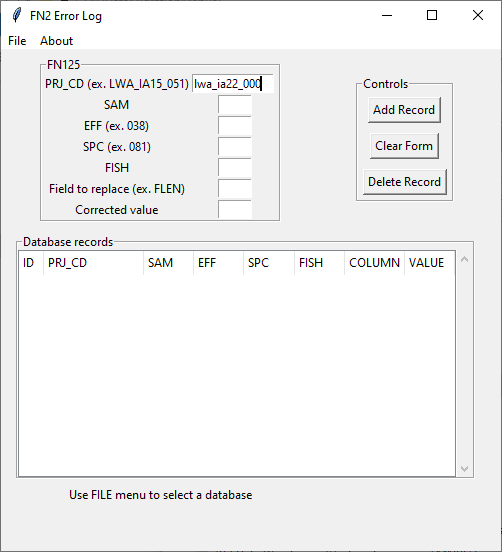
\includegraphics{Figures/DataChangeDB_01.png}
\item
  Create new or open an existing database\\
  On load, you can create a new database or load an existing database from options in the File menu.
  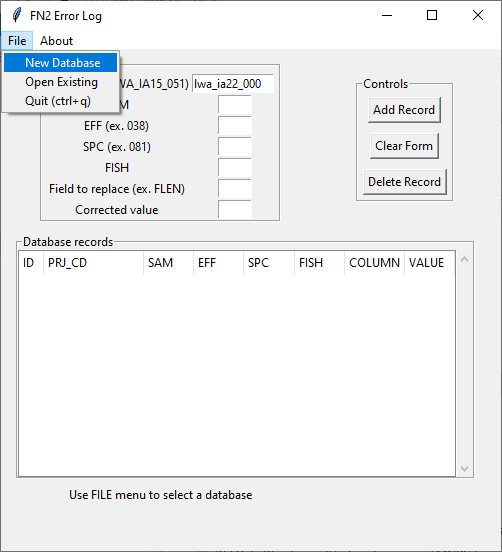
\includegraphics{Figures/DataChangeDB_02.png}
\item
  View current records\\
  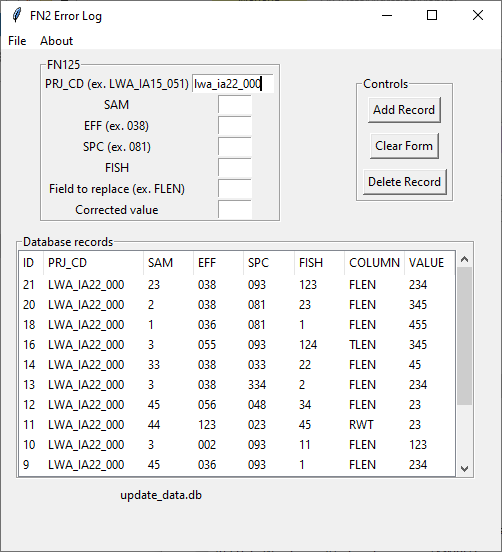
\includegraphics{Figures/DataChangeDB_03.png}
\item
  Add a new data change\\
  You can move between entry boxes using ``TAB''. New records are added to the database via the ``Submit'' button (on click or with ``ENTER'' when highlighted). Currently, errors can only be deleted and not edited (at least not from this GUI - see DBBrowser software to interact with update\_data.db if required). To delete a record, highlight the record in the spreadsheet window that is intended to be deleted and then click ``Delete''.\\
  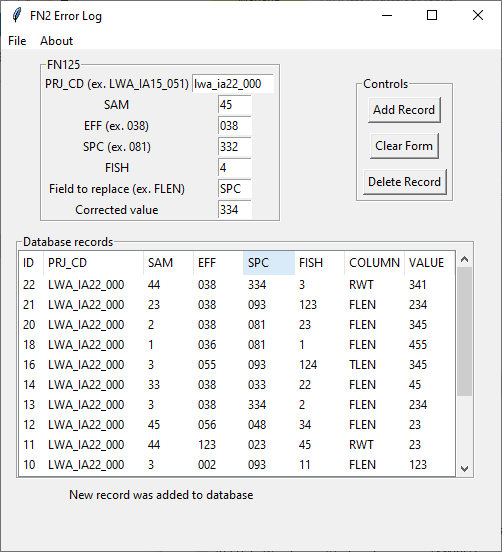
\includegraphics{Figures/DataChangeDB_04.png}
\item
  Delete a record\\
  To delete a record, highlight the record in the spreadsheet window that is intended to be deleted and then click ``Delete''.\\
  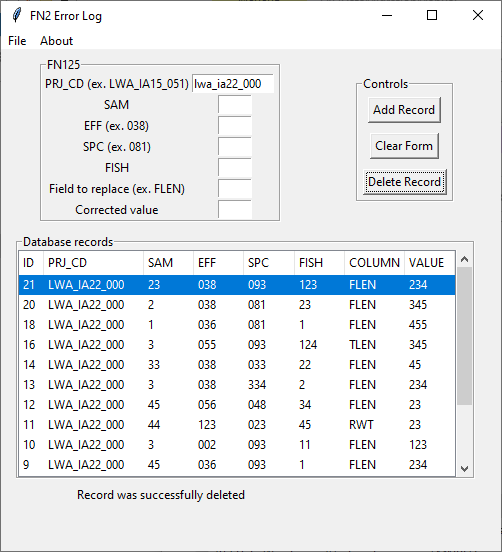
\includegraphics{Figures/DataChangeDB_05.png}
\end{enumerate}

\end{document}
